% !TEX root = ../main.tex
\chapter{Deceptive Box: PANDA meets evasive malware}
\label{chap:5}

As discussed before some particular categories of malware have been developed with specific checks in order to finely fingerprint the environment they are in to check for any sign of virtualization. This means that in order for them to be analyzed some specific virtual machines in which artfacts have been carefully removed and masqueraded are needed.

The goal of this thesis was to develop a set of Panda plugins that can be used to modify the Virtual Machine and Operating System internal state, at run time, in order to hide virtualization artifacts from the system. In this way Evasive Malwares can be run on a Fully Emulated System invalidating their attempts to fingerpint the environment and therefore having them to reveal their real capabilities.
By using Panda for this there are tree advantages: 
\begin{enumerate}
    \item The system can be monitored and modified at run time in order to counter any evasion attempt. 
    \item Due to the fact that it works in full system emulation mode it provides an external view of the system which is segregated but inspectable.
    \item The ability to record and replay allows for a malware to be run once on the live system and then analyzed later.
\end{enumerate}

In the following sections the 4 main contributions will be presented: 

\section{Leveraging panda-re to manipulate the live system}

As widely discussed in the previous chapters \textbf{PANDA} provides many useful features that can be used to modify a running virtual machine. Blindly faking results for different functions or instructions in a system is dangerous as most of them will likely be used by many other programs and giving wrong or arbitrary information might lead to system instability and crashes. Therefore all the plugins written needs to be aware of the target process that needs to be patched.

Instead of hiding every single artifacts left by QEMU on the system the preferred way was to analyze what ParanoidFish and Al-Khaser could find and focus on patching those, subsequently, the plugin can be extended to support different evasion techniques. Due to the nature of this project the resulting plugins will need to be run both on live and replay modes. As a matter of fact the plugins will introduce deep modifications in the system that, due to the way in which the record/replay system works, will need to be run always in order to maintain the integrity of the system during replays.

Some of the hardware based checks can be avoided simply by fine tuning the system, in particular the disk size and RAM size can be adjusted to avoid the detection by setting the RAM to a value greater that 1 GB and the disk to a size greater than 60GB. 

Some of the plugins used to patch the system are designed to be used with the python interface of \textbf{PANDA}, in particular the hooks plugin. Using the python interface will introduce a big overhead in the virtual machine therefore in order to try to reduce it at minimum only it was used only when really necessary (i.e. to perform api hooking). In addition to this it was necessary to create a new \textbf{PANDA} callback in order to have control of the Time Stamp Counter (TSC) during emulation.  

The \textbf{PANDA} plugins directly used for this project are: 

\begin{itemize}
    \item \textbf{osi} or Operating System Introspection was used to interface with the guest Operating System in order to extract for example the list of running programs or the list of loaded libraries. The peculiarity of this plugin is that it puts a layer of abstraction on top of the Operating System making it easy to write a plugin that will then work on all the supported OS.
    
    \item \textbf{syscalls2} is a plugin that provides a Plugin to Plugin interface each time a system call is executed. This plugin uses osi under the hood to perform system calls hooking, this allows for a breakpoint to be placed either when the syscall is executed or when the execution returns from the above sytem call. This latter part is particularly useful when exploring or changing the information returned from a specific syscall.
    
    \item \textbf{hooks} is a plugin that allows the user to specify a address and a function, the function will then be called each time that specific address is reached. This is essentially what a breakpoint is in a debugger.
    
    \item \textbf{hooks2} is the replacement for the hooks plugin however it is not yet completed and not all functionalities are working correctly however it provides some useful PPP interfaces. In particular \lstinline{on_process_start} and \lstinline{on_process_end} were used to execute specific actions when the monitored program was started.
\end{itemize}

Newer versions of windows are not supported by many of these plugins therefore in order to perform the analysis it was decided to use the most recent supported version which is Windows 7 32 bit.
Moreover as cited before, in order for the \textbf{PANDA} plugins to work, it is necessary to use QEMU without the KVM acceleration, this greatly lowers the performance of the system as the instrumentation system introduces a high overhead in the emulation and translation phase. 

\subsection{System call hooking}

The first approach was to write a \textbf{PANDA} plugin to hook system calls associated with typical footprinting performed by evasive malware. This involves having a deep understanding of how the Operating System works and which are its internal structures. A common source of information is the windows registry, there are 3 system calls that are used to access the registry: \lstinline{NtQueryValueKey, NtOpenKey} and \lstinline{NtEnumerateKey}. 

Using the \textbf{syscalls2} plugin different breakpoints were placed on the above mentioned system calls, in particular it was decided to capture the data returned by the above mentioned system calls. As \textbf{PANDA} is based on QEMU/BOCHS these are two of the strings that will be searched in different registry values. \lstinline{NtEnumerateKey} and \lstinline{NtOpenKey} are useful to catch enumeration however, \lstinline{NtQueryValueKey} is the syscall that provides the final string used for detection.

\lstinline{NtQueryValueKey} is the user mode version of \lstinline{ZwQueryValueKey}. This function allows to query the content of a value inside a specific registry key. In particular the key to be queried must have been accessed before with the \lstinline{NtCreateKey} or \lstinline{ZwOpenKey}, these functions will return a \textit{KeyHandle} that identify that specific key and that must be passed as parameter to the \lstinline{NtQueryValueKey} function. In addition to this there are some other values required to properly query the registry key, in particular \textit{ValueName} holds the name of the value to be queried. \textit{KeyValueInformationClass} specify the type of information to be returned and Length specify the length of the output buffer called \textit{KeyValueInformation}. The complete header of such function can be seen in Figure \ref{fig:querykey}.

\begin{figure}[htp]
\centering
\begin{lstlisting}[language=C]
NtQueryValueKey(
  IN HANDLE               KeyHandle,
  IN PUNICODE_STRING      ValueName,
  IN KEY_VALUE_INFORMATION_CLASS KeyValueInformationClass,
  OUT PVOID               KeyValueInformation,
  IN ULONG                Length,
  OUT PULONG              ResultLength );
\end{lstlisting}
\caption{\lstinline{NtQueryValueKey} header}
\label{fig:querykey}
\end{figure}

The \textit{KeyValueInformationClass} is particularly interesting as based on this value the type of information returned inside the \textit{KeyValueInformation} changes.

A common enumeration technique to detect QEMU consists of querying the value \textit{SystemBiosVersion} which is found under the path \lstinline{HKEY_LOCAL_MACHINE\HARDWARE\Description\System} and comparing it with the string \textit{BOCHS}.

In order to patch the above described System Call using \textbf{PANDA} it was necessary to hook the function when it returns, this can be done in the C plugin by registering to use appropriate \textbf{PPP} callback in the \lstinline{init_plugin} section. The implementation can be seen in Figure \ref{fig:pinit}.

\begin{figure}[htp]
\centering
\begin{lstlisting}[language=C]
bool init_plugin(void *self) {
    panda_require("syscalls2");
    [...]
    PPP_REG_CB("syscalls2", on_NtQueryValueKey_return, NtQueryValueKey_return);
    [...]
    return true;
}
\end{lstlisting}
\caption{Snippet of code representing how to hook the \lstinline{NtQueryValueKey} function.}
\label{fig:pinit}
\end{figure} 

The above snippet of code will run the \lstinline{NtQueryValueKey_return} function every time the \lstinline{NtQueryValueKey} returns, it is therefore necessary to have specific checks in place in order to patch the system only when the system call is executed from within a specified program. This has been implemented with a check on the program name or on the PID. Details of the patching function can be seen in Figure \ref{fig:pfun}. The function, after checking if the program running is the one specified for analysis, checks if the queried value is \textit{SystemBiosVersion} then if the value corresponds to \textit{BOCHS} it will replace it with \textit{INTEL}. It is important to note that all the particular structures used by this functions had to be ported from the windows library to this plugin in order for them to be used. Moreover the \lstinline{guest_wstrncpy} function is a helper function used to copy strings from the memory as it can be seen in \ref{fig:gstrin}.

\begin{figure}[htp]
\centering
\begin{lstlisting}[language=C]
void NtQueryValueKey_return(
    CPUState* cpu,
    target_ulong pc,
    uint32_t KeyHandle,
    uint32_t ValueName, 
    uint32_t KeyValueInformationClass,
    uint32_t KeyValueInformation,
    uint32_t Length, 
    uint32_t ResultLength 
    ){ 
    if (check_pid(cpu, tpid, tname)){
        char *name;
        UNICODE_STRING vname;
        name = malloc(1024*sizeof(char));
        panda_virtual_memory_rw(cpu, ValueName, (uint8_t *)&vname, sizeof(UNICODE_STRING), 0); // extract the pointer to string
        guest_wstrncpy(cpu, name, 1024, vname.Buffer); // read the string
        if (strcmp(name, "SystemBiosVersion")==0){
            KEY_VALUE_PARTIAL_INFORMATION rr;
            panda_virtual_memory_rw(cpu, KeyValueInformation, (uint8_t *)&rr, Length, 0);
            if (rr.Data[0]=='B' && rr.Data[8] == 'S'){
                // printf("\n\tPatching BOCHS\n");
                for(int i=0;i<5;i++){
                    char sub[6] = "INTEL";
                    rr.Data[(i*2)] = sub[i];
                }
                panda_virtual_memory_rw(cpu, KeyValueInformation, (uint8_t *)&rr, Length, 1);    
            }
        }
        free(name);
        return;
    }
}
\end{lstlisting}
\caption{Patching the value inside the registry using the \lstinline{NtQueryValueKey_return} function.}
\label{fig:pfun}
\end{figure} 

\begin{figure}[htp]
\centering
\begin{lstlisting}[language=C] 
uint32_t guest_wstrncpy(CPUState *cpu, char *buf, size_t maxlen, target_ulong guest_addr) {
    buf[0] = 0;
    unsigned i;
    for (i=0; i<maxlen; i++) {
        panda_virtual_memory_rw(cpu, guest_addr + 2 * i, (uint8_t *)&buf[i], 1, 0);
        if (buf[i] == 0) {
            break;
        }
    }
    buf[maxlen-1] = 0;
    return i;
}
\end{lstlisting}
\caption{\lstinline{guest_wstrncpy} function implementation.}
\label{fig:gstrin}
\end{figure}

This is an effective method to patch various system calls and can easily be expanded for any other syscall used for Virtualization detection.


\subsection{CPUID hooking}

A robust detection technique employed by malware involve taking advantage of the information provided by the \lstinline{CPUID} instruction as detailed in Section \ref{sec:evmal}. In order to patch the values returned by this instruction it is possible to use a callback already available in \textbf{PANDA}: \lstinline{PANDA_CB_GUEST_HYPERCALL}. This callback is used by the taint plugin to control execution on the host, the way it is implemented is that the callback is triggered each time a \lstinline{CPUID} instruction is generated on the host. Unlike most of the other callbacks that return void this one has bool as return type. This means that the function implementing the callback should return \textit{True} if the hypercall has been processed by the plugin, \textit{False} otherwise. If the function returns \textit{True} \textbf{PANDA} will skip the execution of \lstinline{CPUID} and, instead, assume that the user has handled the instruction and populated the various registers. 

Taking advantage of \lstinline{PANDA_CB_GUEST_HYPERCALL} it was possible to write a function to read the various parameters that \lstinline{CPUID} takes as input in \lstinline{EAX} and then act accordingly. The function can be seen in Figure \ref{fig:cpuidpat}, when the value of \lstinline{EAX} is 1 the function will simply replace the output of the instruction in \lstinline{ECX} with the value 0. This did not pose any problem during the simulation however if the malware needs any of the other information available in the \lstinline{ECX} registry this logic can quickly be modified by xor-ing the content of \lstinline{ECX}, after it is populated by \lstinline{CPUID}, with 0x80000000 (\lstinline{panda.arch.set_reg(cpu, "ECX", ecx^0x80000000)}). In the same way the relevant registers are zeored also for the Hypervisor Brand and CPU Brand instructions.

\todo{put the C plugin instead of the python one}
\begin{figure}[htp]
\centering
\begin{lstlisting}[language=Python] 
@panda.cb_guest_hypercall(name="hyper", procname=process_name)
def tt(cpu):
    eax = panda.arch.get_reg(cpu, "EAX")
    if eax == 1:
        print("CPUID 0x1")
        panda.arch.set_reg(cpu, "ECX", 0) # the endianess is swapped (?)
        return True
    elif eax == 0x40000000:
        print("CPUID Vendor")
        panda.arch.set_reg(cpu, "ECX",0)
        panda.arch.set_reg(cpu, "EDX",0)
        return True
    elif eax >= 0x80000002 and eax<=0x80000004:
        print("CPUID Brand")
        panda.arch.set_reg(cpu, "EAX",0)
        panda.arch.set_reg(cpu, "EBX",0)
        panda.arch.set_reg(cpu, "ECX",0)
        panda.arch.set_reg(cpu, "EDX",0)
        return True
    return False
\end{lstlisting}
\caption{CPUID patching}
\label{fig:cpuidpat}
\end{figure}


\subsection{API hooking}

Patching other virtualization artifacts such as library calls and RDTSC instructions is a more complex task as there are no available plugins or callbacks specific for such events. In order to perform API hooking It was decided to switch to python this, as mentioned before, has some other advantages such as the ability to run a complete simulation by having complete control over the virtual machine from the python script. Moreover one of the advantages of the python library is that it has a builtin mechanism for running callbacks only when a specific program is running simply by passing the process name to the python function. In addition to this the pypanda interface supports enabling and disabling callbacks dynamically, this mechanism helps to mitigate some of the overhead introduced by enabling relevant function only when specific events happen on the system.

It must be noted that all the flexibility provided by python on the management and interaction side is at the cost of performance therefore, simulations run using the python script have a much lower performance than the native ones. 

Pypanda uses Python decorators\footnote{\url{https://wiki.python.org/moin/PythonDecorators}} to implement callbacks and PPP functions, a decorator is a way of altering the functionality of functions, methods or classes without having to directly interact with the source code and avoiding repetitions. In Python decorators are defined with the \lstinline{@} symbol at the beginning of the line, the following function will then alter, replace or extend the one specified after the \lstinline{@}. In this particular case decorators let the user specify the function that should be run when the event defined by the callback happens. 

This python plugin is a bit more complicated as it requires to hook some specific functions in a library on the system. As the libraries are loaded at a different address each time it is necessary to first find out the right address at which the library will be loaded, then the offset of the function to be hooked must be added to the base address of library and finally it is possible to set the desired breakpoint. It must be noted that in order for the breakpoint to work the code of the library must have been already loaded in memory. 

The steps taken in this plugin to correctly place hooks and patch artifacts in the system can be sum up in the following points:

\begin{itemize}
    \item Find the offset of the function to be hooked in the right library. This can be done offline as it involves statically inspecting the library.
    \item Find the base address at which the library is loaded in the system at run time.
    \item Find out when the code of the library is loaded in virtual memory.
    \item Place the hook at base address+offset.
\end{itemize}

As the \lstinline{GetSystemInfo} function from \textit{kernel32.dll} is the one called by ParanoidFish in order to get the number of processors, the process described in the rest of the paragraph is focused on this function. However, the process is identical for any other function and library.

In order to place the hook in the correct place it is important to first find out the offset of the function to be hooked inside the library, this can be easily accomplished by opening the dll with pestudio which will give the offset of all the functions exported by the dll as it can be seen in Figure \ref{fig:pestudio}. In the case of \lstinline{GetSystemInfo} on the version of \textit{kernel32.dll} running on the test system the offset is \lstinline{0x53728}.

\noindent
\begin{figure}[htp]
\centering
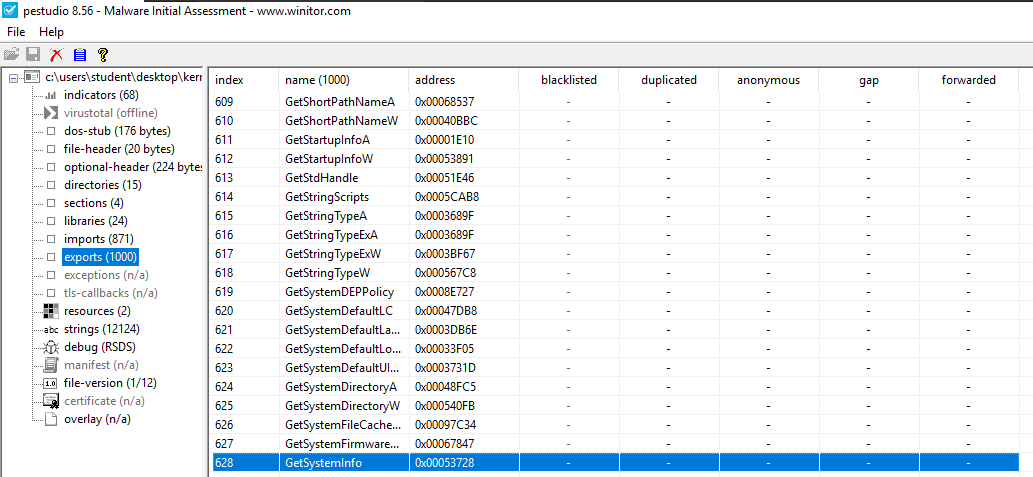
\includegraphics[width=\linewidth]{images/pestudio.png}
\caption{Finding offset of functions using pestudio}
\label{fig:pestudio}
\end{figure}


Subsequently the base address of the libraries loaded in the system must be found. In order to do this the pypanda helper function \lstinline{panda.get_mappings(cpu)} was used. Such function is based on the osi plugin and will return as output a dictionary containing the libraries loaded in the system in that precise moment. This implies that the function will return the libraries loaded by the executable running at the time it was called. By combining it with the syscalls2 plugin it is therefore possible to find out when a specific program is starting to load libraries in the system. In particular the following approach was used: leveraging syscalls2 PPP a callback was placed on the execution of \lstinline{NtMapViewOfSection}. This system call is used by a process to map a file into its memory address space, which is the case of loading libraries from disk. The function designed to execute when the syscall takes place can be seen in Figure \ref{fig:ntmap}. In there if the process running matches the target one the loaded libraries will be extracted and compared against the one containing the api function to be hooked. Once a match is found the function will in turn enable a memory callback \lstinline{cb1} of type \lstinline{PANDA_CB_VIRT_MEM_BEFORE_READ} and then disable itself.

\begin{figure}[htp]
\centering
\begin{lstlisting}[language=Python] 
@panda.ppp("syscalls2", "on_NtMapViewOfSection_return", name="ntmap")
def ntmap(cpu, pc, SectionHandle,  ProcessHandle, BaseAddress, ZeroBits, CommitSize, SectionOffset, ViewSize, InheritDisposition, AllocationType, Win32Protect):
    proc = panda.get_process_name(cpu)
    print(proc)
    if proc == process_name:
        mappings = panda.get_mappings(cpu)
        for mapping in mappings:
            print(
                "Name: "+ffi.string(mapping.name).decode(),
                "Base: 0x{:x} Size: 0x{:x}".format(mapping.base,mapping.size)
            )
            if ffi.string(mapping.name).decode().lower() == "kernel32.dll":
                global base
                base = mapping.base
                global si
                si = mapping.size
                print("Enabling memory callback")
                panda.enable_callback("cb1")
                print("Disabling MapViewOfSections hook")
                panda.disable_ppp("ntmap")
\end{lstlisting}
\caption{\lstinline{NtMapViewOfSection} hooking}
\label{fig:ntmap}
\end{figure}

The memory callback can be seen in Figure \ref{fig:cb1}. It is necessary as when the \lstinline{NtMapViewOfSection} function is called the library is not yet loaded into the reserved virtual memory and therefore placing an hook at an address in that range will not work as it will be overwritten when the content of the dll is loaded. Instead, by monitoring the reserved portion of memory for a read operation, we will be sure that when the read takes place the code will have been loaded in memory and therefore the hook can be place safely. 

\begin{figure}[htp]
\centering
\begin{lstlisting}[language=Python] 
@panda.cb_virt_mem_before_read(name="cb1", procname=process_name, enabled=False)
def virt_mem_after_read(cpu, pc, addr, size):
    if (addr > base and addr < base+si) and base !=0 and si !=0:
        panda.update_hook("sysinfohook",base+0x53728) # offset of GetSystemInfo
        panda.enable_hook("sysinfohook")
        panda.disable_callback("cb1")
        
\end{lstlisting}
\caption{memory callback cb1}
\label{fig:cb1}
\end{figure}

The\lstinline{GetSystemInfo} function is actually really straight forward as it takes in input a pointer to a \lstinline{SYSTEM_INFO} structure that will hold the results, the fields of the structure can be seen in Figure \ref{fig:sysinfo}.

\begin{figure}[htp]
\centering
\begin{lstlisting}[language=C++] 
typedef struct _SYSTEM_INFO {
  union {
    DWORD dwOemId;
    struct {
      WORD wProcessorArchitecture;
      WORD wReserved;
    } DUMMYSTRUCTNAME;
  } DUMMYUNIONNAME;
  DWORD     dwPageSize;
  LPVOID    lpMinimumApplicationAddress;
  LPVOID    lpMaximumApplicationAddress;
  DWORD_PTR dwActiveProcessorMask;
  DWORD     dwNumberOfProcessors;
  DWORD     dwProcessorType;
  DWORD     dwAllocationGranularity;
  WORD      wProcessorLevel;
  WORD      wProcessorRevision;
} SYSTEM_INFO, *LPSYSTEM_INFO;
\end{lstlisting}
\caption{\lstinline{STYSTEM_INFO} structure.}
\label{fig:sysinfo}
\end{figure}

The content of this structure will be populated after the function executes therefore in order to correctly modify the \lstinline{dwNumberOfProcessors} field, which is the one checked by ParanoidFish, it is necessary to obtain the return address at which the function will jump after the execution. In this way the structure will have already been populated and the fields can be safely modified.

This can be achieved by saving the return address placed on the stack when the function is called and setting a breakpoint on such address. In this way the address of the structure can be extracted from the stack once the function returns and then the \lstinline{dwNumberOfProcessors} field patched.  


As mentioned before the use of Python provides great flexibility not only in plugin writing but also on the automation side. In order to automate the analysis the record and replay actions have been automated inside the python script. To achieve this the hooks2 plugin was used, such plugin is designed to substitute the hooks one. Although it is not yet finished it already provides some useful callbacks, in particular the \lstinline{on_process_start} and \lstinline{on_process_end} callbacks have been used to start and stop the recording. Some checks have been put in place in order to execute the code only if the process is the one monitored and only if the script is being run on a live system. Details of such functions can be seen in \ref{fig:startstop}

\begin{figure}[htp]
\centering
\begin{lstlisting}[language=Python] 
# Only used to take recordings of patched sessions
@panda.ppp("hooks2", "on_process_start")
def rec(cpu, procname, asid, pid):
    print(ffi.string(procname).decode())
    if ffi.string(procname).decode() == process_name:
        print(ffi.string(procname).decode()," Started!")
        if not rep:
            panda.run_monitor_cmd("begin_record rec")

@panda.ppp("hooks2", "on_process_end")
def end_rec(cpu, procname, asid, pid):
    if (ffi.string(procname).decode() == process_name) and not rep:
        panda.disable_callback("hyper")
        panda.disable_hook("sysinfohook")
        panda.disable_hook("patchsysinfo")
        panda.disable_ppp("ntmap")
        panda.run_monitor_cmd("end_record")
\end{lstlisting}
\caption{functions used to start and stop the recording.}
\label{fig:startstop}
\end{figure}


\subsection{Faking time results}

Another important fingerprinting technique consists in checking the Time Stamp Counter (TSC) of the system in order to check the time elapsed between different instructions. Most CPUs provide a dedicated instruction to access the TSC called RDTSC, the most common fingerprinting techniques involve checking the time elapsed between two subsequent execution of RDTSC or fingerprinting the time it takes for a VM Exit to happen. A simple VM exit can be generated with CPUID as it is a privileged instruction as explained in Chaper \ref{chap:2}.

One of the limitation of \textbf{PANDA} is that it does not provide a callback able to intercept all the types of hypervisor call such as CPUID and RDTSC but, instead, CPUID is the only one associated with \lstinline{PANDA_CB_GUEST_HYPERCALL}. Therefore, in order to manipulated the TSC of the emulated system, it was necessary to introduce some modifications inside the \textbf{PANDA} code base an in particular to add a new callback specifically dedicated to the RDTSC instruction. 

\textbf{PANDA} already provides the possibility to create Plugin to Plugin interfaces which are particular types of callbacks. However, those can only be based on functions already exposed by the \textbf{PANDA} api which does not provide the necessary level of control over the emulated architecture. Instead a new "native" callback was created for TSC handling named \lstinline{PANDA_CB_RDTSC}. 

In order to do this it is first necessary to understand how QEMU handles the TSC counter for the guest Operating System and how \textbf{PANDA} callbacks works internally. On this last point it was not possible to find any reference about extending \textbf{PANDA} functionalities inside the documentation and therefore the source code had to be manually interpreted in order to find out where the modifications should take place.

The files involved in the creation of ``native'' callbacks are the following: 

\begin{itemize}
    \item \lstinline{./panda/include/panda/callbacks/cb-defs.h} this header file holds the declaration of the \lstinline{panda_cb_type} type as well as a union of all possible callback function types.
    
    The modifications introduced in this file in order to support a new callback can be seen in Figure \ref{fig:mod1}.
    
    \begin{figure}[htp]
    \centering
    \begin{lstlisting}[language=C]
    typedef enum panda_cb_type {
        [...]
        PANDA_CB_RDTSC, // <- New callback
        PANDA_CB_LAST
    } panda_cb_type;
    
    // Union of all possible callback function types
    typedef union panda_cb {
        [...]
        bool (*rdtsc)(CPUState *env, uint64_t val); // <- New callback
    } panda_cb;
    \end{lstlisting}
    \caption{\textbf{cb-defs.h} modifications}
    \label{fig:mod1}
    \end{figure}
        
    \item \lstinline{./panda/include/panda/callbacks/cb-support.h} this header file contains the signatures for the \textbf{PANDA} callback helper functions. The helpers essentially iterate over the list of registered callbacks and invoke them with the appropriate arguments. In this file was added the signature of the new callback helper function: 
    \lstinline{bool panda_callbacks_rdtsc(CPUState *env, uint64_t val);}
    
    \item \lstinline{./panda/src/cb-support.c} this file contains the description of how the callback should be build. In particular teh \lstinline{cb-macros.h} file defines some custom functions: \lstinline{MAKE_CALLBACK} and \lstinline{MAKE_REPLAY_ONLY_CALLBACK} that will take care of generating the callback helper function. The following line was added to this file: \lstinline{MAKE_CALLBACK(bool, RDTSC, rdtsc, CPUState*, env, uint64_t, val);}
    
\end{itemize}

Once the callback has been defined in the above mentioned \textbf{PANDA} files it can be used inside the code. In particular in order for a callback to work it must specified at which point of the emulation the callback should be invoked. For example the \lstinline{PANDA_CB_BEFORE_BLOCK_EXEC}, which is called before a basic block is executed(Figure \ref{fig:calls}), is implemented with the \lstinline{panda_callbacks_before_block_exec(CPUState *env, TranslationBlock *tb);} which is then called in the \lstinline{cpu_tb_exec} function inside the main emulator file (\lstinline{./cpu-exec.c}).

In the case of RDTSC it was first necessary to track down how QEMU manages such counter in the virtual CPU. There are 3 different places in which the TSC counter is managed:

\begin{itemize}
    \item The \lstinline{cpu_get_ticks} function returns the time elapsed inside the VM. This function is implemented in \lstinline{./cpus.c} and is directly connected to the host one as it calls the \lstinline{cpu_get_host_ticks}.
    \item The above function is then called in the \lstinline{cpu_get_tsc} which is the function called in the i386 cpu implementation to handle the tsc counter. 
    \item Lastly in the \lstinline{./target/i386/misc_helper.c} there is a function called \lstinline{helper_rdtsc} which takes care of handling the RDTSC instruction inside the guest. This appears to be the best place in which to place the callback function. As a matter of fact this is the same file in which the CPUID hooking function is placed. 
\end{itemize}

The logic to implement this callback is partially inspired to the one used in the \lstinline{PANDA_CB_GUEST_HYPERCALL}. The \lstinline{panda_callbacks_rdtsc} function is called inside \lstinline{helper_rdtsc}, the return type of the callback is boolean meaning that the plugin using it can signal if RDTSC has been handled or not. In particular, if the callback returns \textit{true}, the values of TSC are not copied in the RAX and RDX registers but it is assumed that the plugin has taken care of populating the registers with the correct value. On the other hand, if the callback returns \textit{false}, the normal execution continues and the registers are populated with the correct values. 

The TSC value is also passed to \lstinline{panda_callbacks_rdtsc} under the \lstinline{val} parameter. In this way the plugin has a direct and convenient access to the Timestamp that would have been used to populate the registers and can manipulate it accordingly.

The function responsible to patch RDTSC in the plugin can be seen in Figure \ref{fig:rdtscpatch}. The approach taken here was to bring down TSC difference by dividing the value by an arbitrary number. Such number was calculated empirically and depends is dependant on the system running and on the number of plugins loaded as the execution time will vary based on the load of the emulated system.

\begin{figure}[htp]
\centering
\begin{lstlisting}[language=C]
bool rdtsc(CPUState *cpu, uint64_t val){
    if (rdtsc_patch==1){
        if (check_pid(cpu,tname)){ // we need this here otherwise it will segfault
            val=val/10000;
            EAX = (uint32_t)(val);
            EDX = (uint32_t)(val >> 32);
            printf("[DEBUG] rdtsc patched!\n");
            return true;
        }
    }
    return false;
}
\end{lstlisting}
\caption{\textbf{cb-defs.h} modifications\daniele{Nicer caption?}}
\label{fig:rdtscpatch}
\end{figure}

This plugin can also be combined with CPUID in order to specifically patch RDTSC if it is called to fingerprint the time taken by a VM Exit to be handled. 

In order to test if this plugin was working and also test the performances of the fully emulated system it was necessary to write a custom test program. This can be found in Figure \ref{fig:rdttest}. The goal was to check the difference in time between two different calls of RDTSC in order to:

\begin{enumerate}
    \item Define a baseline of the time taken by instructions to be executed on a bare metal system Figure \ref{fig:bmetal}.
    \item Determine the time it takes to execute the same instruction under full system emulation Figure \ref{fig:rdtsc1}(a). This is particularly challenging as the more plugins are used in the system the more it takes for the entire emulation to run. The results in the Figure \ref{fig:rdtsc1}(a) were obtained with all the above created plugins loaded. 
\end{enumerate}


\begin{figure}[htp]
\centering
\begin{lstlisting}[language=C]
#include <windows.h>
#include <stdio.h>

void test1(){
    unsigned long long ret, ret1, ret2;
	unsigned eax, edx;
    for (int i=0;i<11;i++){
        __asm__ volatile("rdtsc" : "=a" (eax), "=d" (edx));
        ret  = ((unsigned long long)eax);
        __asm__ volatile("rdtsc" : "=a" (eax), "=d" (edx));
        ret1  = ((unsigned long long)eax);

        printf("First call %llu\n",ret);
        printf("Second call %llu\n",ret1);

        printf("Difference %llu\n",ret1-ret);
    }

    __asm__ volatile("rdtsc" : "=a" (eax), "=d" (edx));
    ret  = ((unsigned long long)eax) | (((unsigned long long)edx) << 32);
	
	__asm__ volatile("cpuid" : /* no output */ : "a"(0x00));
	
	__asm__ volatile("rdtsc" : "=a" (eax), "=d" (edx));
	ret2  = ((unsigned long long)eax) | (((unsigned long long)edx) << 32);
    printf("VM exit %llu\n",ret2-ret);
}



int main(){
    printf("Calling test1\n");
    test1();
    getchar();
    return 0;
}
\end{lstlisting}
\caption{RDTSC testing program}
\label{fig:rdttest}
\end{figure}

\begin{figure}%
    \centering
    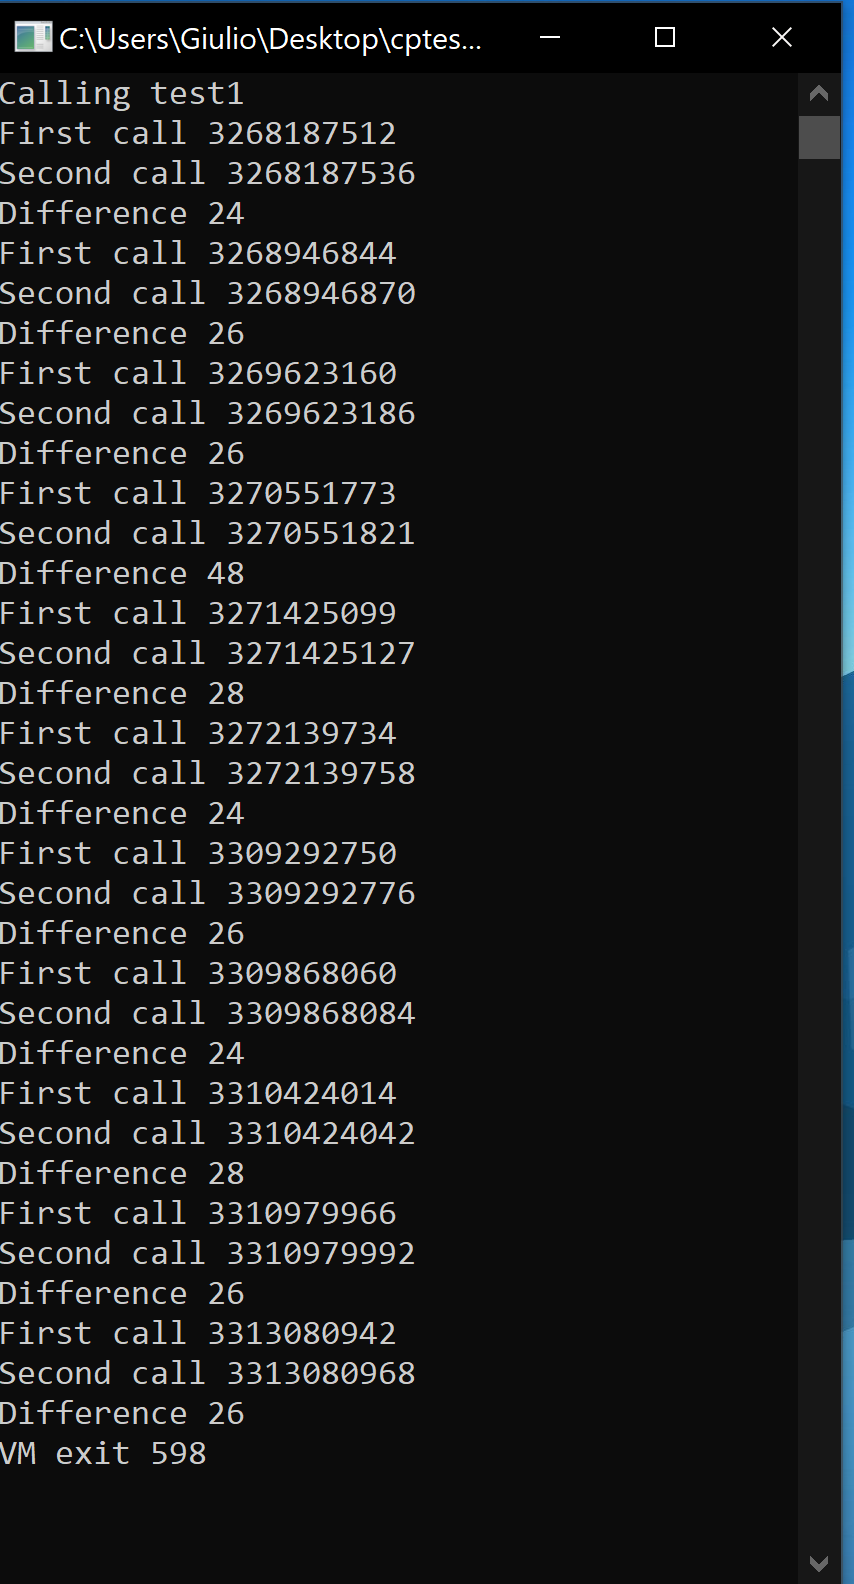
\includegraphics[width=0.6\linewidth]{images/bmetal.PNG}%
    \caption{Results of running RDTSC test program on a bare metal machine}%
    \label{fig:bmetal}%
\end{figure}

\begin{figure}%
    \centering
%    \iffalse % [Daniele] it won't compile on my machine so I use this trick
    \subfloat[\centering vanilla system]{{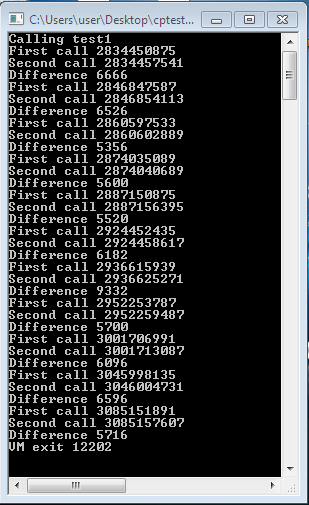
\includegraphics[width=0.5\linewidth]{images/cptest2.png} }}%
    \subfloat[\centering plugin]{{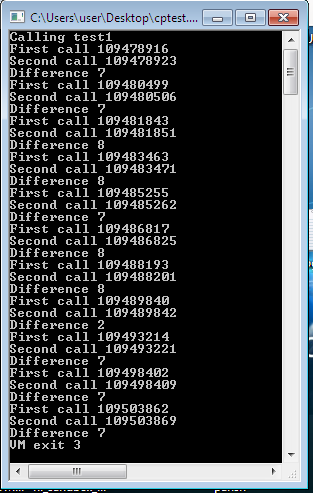
\includegraphics[width=0.5\linewidth]{images/cptest3.png} }}%
%    \fi
    \caption{Results of running RDTSC without the patch (a) and with the \lstinline{timing_patch} plugin applied (b)}%
    \label{fig:rdtsc1}%
\end{figure}

Lastly in Figure\ref{fig:rdtsc1}(b) it is possible to see how the plugin is able to effectively patch the RDTSC instruction faking the result of that instruction by overwriting the values in the EAX and EDX registries. 

\section{Results}

In order to validate the newly created plugins it was decided to use the two most common and complete tools for assessing malware analysis environment against common evasion techniques: ParanoidFish and Al-Khaser.

In Figure \ref{fig:res} it is possible to see how the execution of Paranoid Fish on a system with all plugins enabled compares to a vanilla execution. 

In Figure \ref{fig:res1} it is possible to see how the execution of Al-Khaser compares to a vanilla execution. 


It is possible to see how some tests are still flagged as failed. For example the disk one can easily be fixed by creating a bigger virtual hard disk. The WMI ones are particularly interesting as it requires a deep understanding of how WMI is treated inside Windows and how it can be patched. A detailed discussion on this can be found in the next chapter. 


\daniele{Come up with clever ideas to extend this section or we will have big trouble :-) For instance start explaining how you defeat some evasions using the different components you developed, and how sometimes different components cooperate (rdtsc+cpuid VM exit case right?). You can show some snippets of the code from either suite (e.g. 2 from Al-Khaser and 1 from Paranoid fish) and detail how your plugin(s) craft the right fake answer.}
